\documentclass[tikz,border=8pt]{standalone}
\usepackage{amsmath,amssymb}
\usetikzlibrary{arrows.meta,calc}

\begin{document}
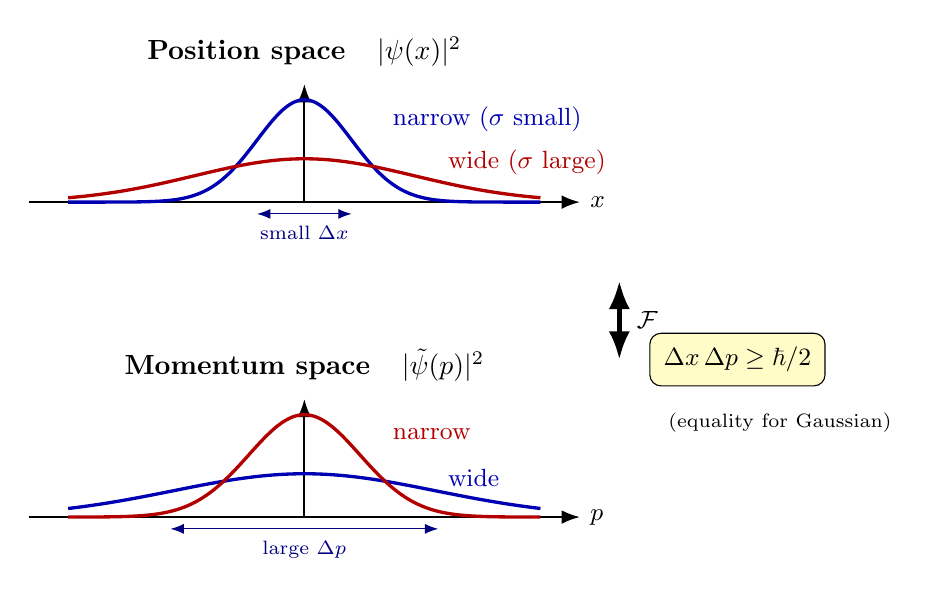
\begin{tikzpicture}[>=Latex]

  % TOP: position space
  \begin{scope}[yshift=2.5cm]
    \node[font=\bfseries, anchor=south] at (0, 1.6) {Position space\quad $|\psi(x)|^2$};

    \draw[->, thick] (-3.5, 0) -- (3.5, 0) node[right, font=\small]{$x$};
    \draw[->, thick] (0, 0) -- (0, 1.5);

    % narrow gaussian (sigma=0.6)
    \draw[blue!70!black, very thick, smooth, samples=140, domain=-3:3]
      plot(\x, {1.3*exp(-\x*\x/0.72)});
    \node[font=\small, blue!70!black, anchor=west] at (1.0, 1.05) {narrow ($\sigma$ small)};

    % wide gaussian (sigma=1.4)
    \draw[red!70!black, very thick, smooth, samples=140, domain=-3:3]
      plot(\x, {0.55*exp(-\x*\x/3.92)});
    \node[font=\small, red!70!black, anchor=west] at (1.7, 0.5) {wide ($\sigma$ large)};

    \draw[<->, thin, blue!50!black] (-0.6, -0.15) -- (0.6, -0.15);
    \node[font=\scriptsize, blue!50!black, anchor=north] at (0, -0.18) {small $\Delta x$};
  \end{scope}

  % Fourier arrow
  \begin{scope}[yshift=1.0cm]
    \draw[<->, ultra thick] (4.0, 0.5) -- (4.0, -0.5);
    \node[font=\small, anchor=west] at (4.1, 0) {$\mathcal F$};
  \end{scope}

  % BOTTOM: momentum space
  \begin{scope}[yshift=-1.5cm]
    \node[font=\bfseries, anchor=south] at (0, 1.6) {Momentum space\quad $|\tilde\psi(p)|^2$};

    \draw[->, thick] (-3.5, 0) -- (3.5, 0) node[right, font=\small]{$p$};
    \draw[->, thick] (0, 0) -- (0, 1.5);

    % wide momentum (corresponds to narrow x — 1/sigma=1.67)
    \draw[blue!70!black, very thick, smooth, samples=140, domain=-3:3]
      plot(\x, {0.55*exp(-\x*\x/5.56)});
    \node[font=\small, blue!70!black, anchor=west] at (1.7, 0.5) {wide};

    % narrow momentum (corresponds to wide x — 1/sigma=0.71)
    \draw[red!70!black, very thick, smooth, samples=140, domain=-3:3]
      plot(\x, {1.3*exp(-\x*\x*1.0)});
    \node[font=\small, red!70!black, anchor=west] at (1.0, 1.05) {narrow};

    \draw[<->, thin, blue!50!black] (-1.7, -0.15) -- (1.7, -0.15);
    \node[font=\scriptsize, blue!50!black, anchor=north] at (0, -0.18) {large $\Delta p$};
  \end{scope}

  % Right side equation
  \node[font=\small, fill=yellow!22, draw, rounded corners, inner sep=5pt] at (5.5, 0.5)
    {$\Delta x\,\Delta p \ge \hbar/2$};
  \node[font=\scriptsize, anchor=west] at (4.5, -0.3) {(equality for Gaussian)};
\end{tikzpicture}
\end{document}
